Un tanque de capacidad $100\,\mathrm L$ contiene inicialmente $50\,\mathrm L$ de agua pura. Desde $t=0$ entra una disolución de $2\,\mathrm{g/L}$ a $5\,\mathrm{L/min}$. En $t=3$ minutos comienza a salir mezcla homogénea a $6\,\mathrm{L/min}$, mientras continúa la entrada. Suponga mezcla perfecta y volúmenes aditivos; el modelo de mezcla termina al vaciarse el tanque.

\begin{enumerate}[label=(\alph*),ref=\alph*,leftmargin=*]
\item Determine el volumen y la cantidad de sal en cada régimen.
\item Obtenga la concentración y explique el comportamiento al final del intervalo físico. ¿Se puede interpretar aquí un límite cuando $t\to\infty$?
\item Halle el máximo de la cantidad de sal, el instante y el volumen correspondientes.
\end{enumerate}

\Needspace{6.68cm}
\begin{center}
\begin{minipage}{\linewidth}
\centering
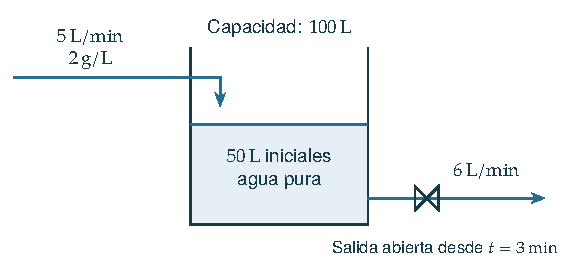
\includegraphics[width=10.94cm]{assets/M2-E0030-setup.pdf}\par
\smallskip{\small Entrada continua y apertura retardada de la salida.\par}
\end{minipage}
\end{center}
